\section{Introduction}
\label{sec:intro}

\begin{figure*}[t]
\centering
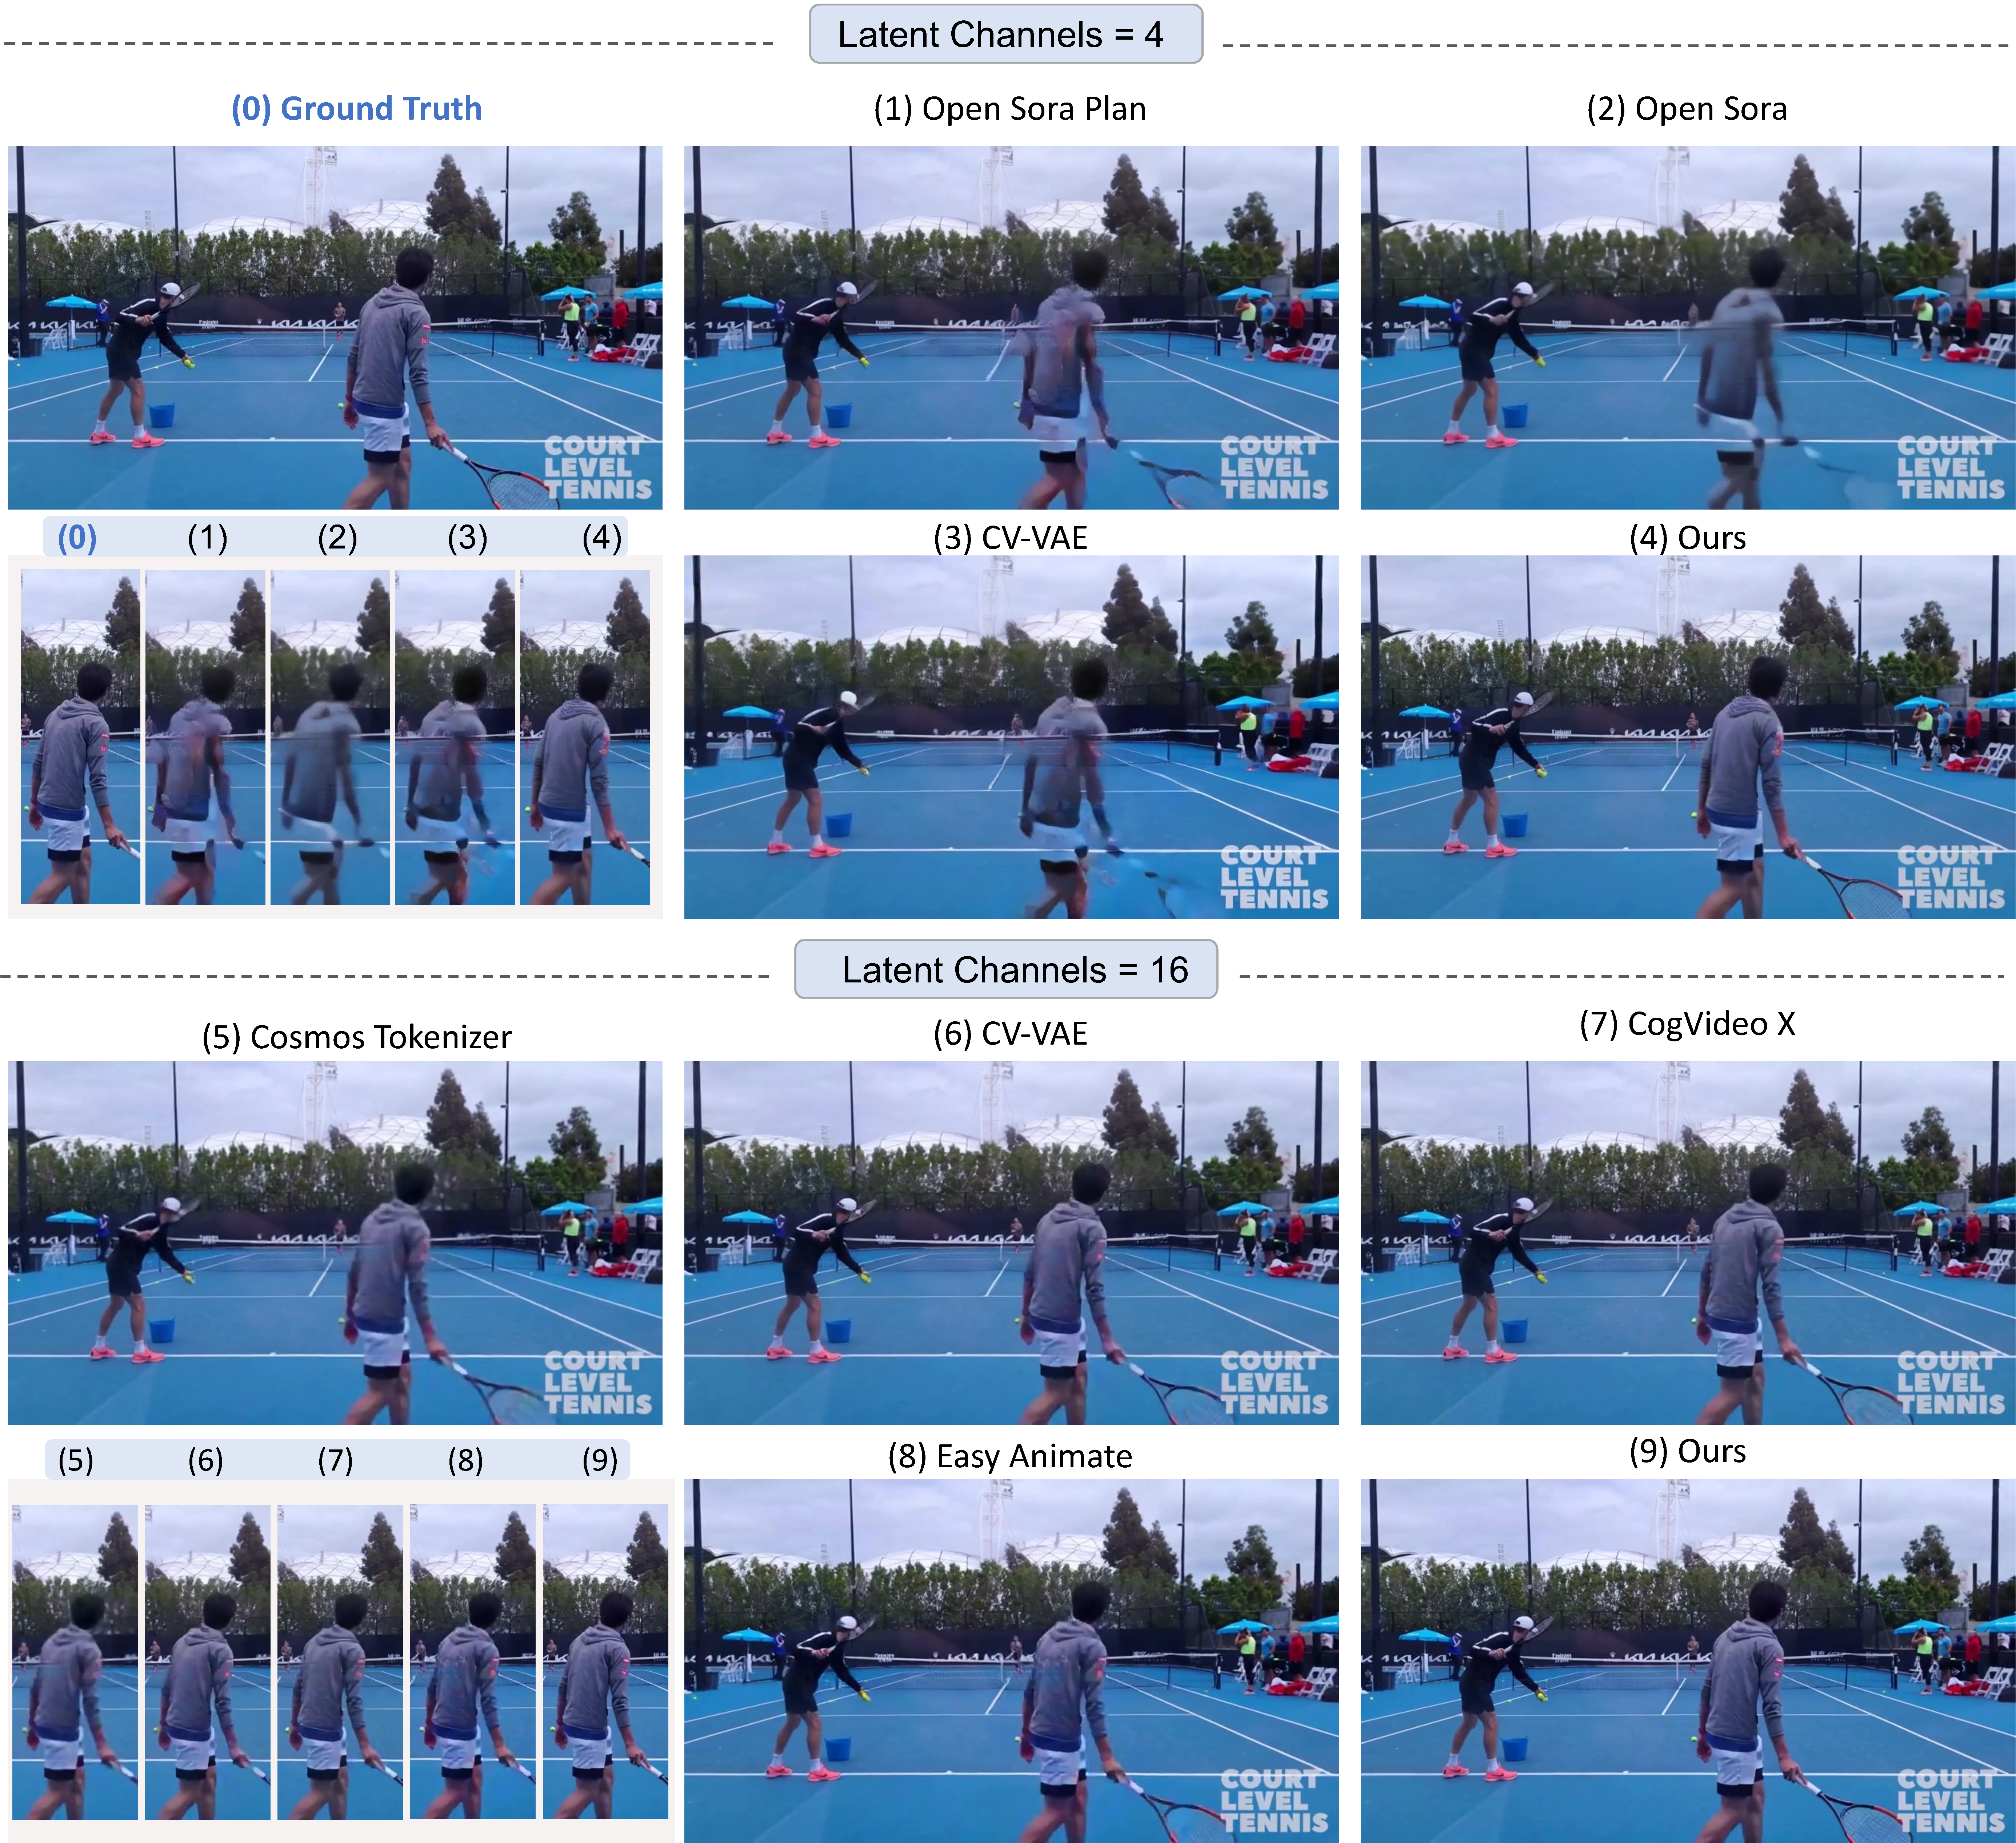
\includegraphics[width=1.0\textwidth]{images/fig1-4and16.pdf}
\caption{
Our reconstruction results compared with a line of three recent strong baseline approaches. 
The ground truth frame is (0). Our model significantly outperforms previous methods, especially under large motion scenarios such as people doing sports.
}
\label{fig:teaser}
\vspace{-3mm}
\end{figure*}



Given the significant attention in the field of video generation, Latent Video Diffusion Models (LVDMs)~\cite{blattmann2023stable, blattmann2023align, he-lvdm, zhou2022magicvideo, he-videocrafter1} have emerged as a popular framework. They have been successfully applied to powerful text-to-video models such as Sora~\cite{videoworldsimulators2024}, VideoCrafter~\cite{he-videocrafter1, chen2024videocrafter2overcomingdatalimitations}, and CogVideoX~\cite{yang2024cogvideox}.
Different from directly generating video pixels, LVDMs generate latent video representations in a compact latent space. This is achieved by first training a Video VAE to encode videos into this latent space.
%
Thus, Video VAE, as a key and fundamental component of LVDMs, has attracted great attention recently.
%
An effective Video VAE can help to reduce the training costs of video diffusion models while improving the final quality of the generated videos.
%
Initially, a series of studies adopt the image VAE from Stable Diffusion~\cite{rombach2022high} for video generation tasks, including AnimateDiff~\cite{guoanimatediff}, MagicVideo~\cite{zhou2022magicvideo}, VideoCrafter1~\cite{he-videocrafter1}, and VideoCrafter2~\cite{chen2024videocrafter2overcomingdatalimitations}. 
%
However, directly adopting an image VAE and compressing video on a frame-by-frame basis leads to temporal flickering due to the lack of temporal correlation. Additionally, the information redundancy along the temporal dimension is not reduced, leading to low training efficiency for subsequent latent video diffusion models.
%
From the introduction of Sora, which compresses videos both temporally and spatially through a Video VAE, a series of studies have emerged that aim to replicate Sora and train their own Video VAEs, including Open Sora~\cite{opensora}, Open Sora Plan~\cite{pku_yuan_lab_and_tuzhan_ai_etc_2024_10948109}, CV-VAE~\cite{zhao2024cv}, CogVideoX~\cite{yang2024cogvideox}, EasyAnimate~\cite{xu2024easyanimatehighperformancelongvideo}, and Cosmos Tokenizer~\cite{cosmos_token}.
%
However, the performance of the current video VAE suffers from many problems, including motion ghost, low-level temporal flickering, blurring (faces, hands, edges, texts), and motion stuttering (lack of correct temporal transition).
% as shown in Fig.~\ref{fig:teaser}.


In this work, we propose a novel cross-modal Video VAE with better spatial and temporal modeling ability in order to solve the aforementioned challenge problems and obtain a robust and high-quality Video VAE.
%
First, we examine different designs for spatial and temporal compression, including simultaneous spatial-temporal (ST) compression and sequential ST compression. 
%
We observed that simultaneous ST compression achieves better low-level temporal smoothness and texture stability, while sequential ST compression achieves better motion recovery, particularly in scenarios of large motion.
%
Thus, we propose a novel architecture that integrates the advantages of both methods and enables effective video detail and motion reconstruction.

Second, we observed that the normally used datasets for text-to-video generation contain text-video pairs. 
Also, during decoding, a text description exists as it serves as the input in the first stage, \textit{i.e.}, the video latent generation stage.
%
To this end, we integrate the text information into the encoding and decoding procedure and propose the first Cross-modal Video VAE.
%
We carefully study how text guidance can be integrated into the spatiotemporal backbone and the mechanism of spatial and temporal semantic guidance. 

In addition, our cross-modal video VAE supports image-video joint training.
To achieve this, we design our network with a fully spatiotemporal factorized architecture, and we feed image and video batches alternately to the network. 
%
During image batches, the data only forwards the spatial part of the network, with the temporal modules being skipped. During video batches, the video forwards both spatial and temporal modules. We also demonstrate that image joint training is crucial for training a video VAE.
%
In summary, our contributions are as follows:
\begin{itemize}
    \item We propose an effective and robust Video VAE, conduct extensive experiments, and achieve the state-of-the-art.
    \item We propose an optimal spatiotemporal modeling approach for Video VAE.
    \item We propose the first cross-modal video VAE that leverages the information from other modalities, i.e., text descriptions, to the best of our knowledge.
    \item Our video VAE is designed and trained to be versatile to conduct both image and video compression. 
\end{itemize}

